\chapter{Fundamentação Teórica}\label{chp:LABEL_FUND_TEORICA}

Tendo em vista que o foco principal desse estudo é a comparação entre a esteira de renderização vigente e sua versão aprimorada utilizando mesh shaders em aplicações dinâmicas, Este capitulo abordará os conceitos básicos por trás da esteira de renderização atual e os novos módulos maleáveis de programação em contexto gráfico.

\section{Esteira de renderização}\label{sec:LABEL_CHP_1_SEC_PIPELINE_RENDERIZACAO}

O termo \textit{renderizar} remete-se à ideia de sintetizar mídias processadas através do computador. Em computação gráfica, este termo é utilizado para se referir à construção de imagens digitais. A esteira, ou, \textit{pipeline} de renderização, consiste em uma sequencia de etapas fixas e programáveis cujo o propósito é desenhar um ou mais objetos em uma cena.

A técnica mais utilizada para a renderização de imagens em aplicações em tempo real é a \textit{rasterização}. A rasterização consiste na transformação de uma imagem vetorial, montada através de um conjunto de vetores denominados de \textit{vértices}, em um conjunto de \textit{rasters} (ou pixels\footnote{menor ponto de uma imagem bidimensional convencional}). Um vértice é uma estrutura de dados que representa o menor ponto no espaço. Além de suas coordenadas, vértices podem armazenar outras informações como cor, vetor normal, coordenada de textura, etc. O produto da rasterização é escrito no \textit{frame buffer}. O frame buffer é uma região de memória que armazena as informações necessárias para a exibição dos dados computados em um dispositivo de saída de vídeo.

Durante a renderização de uma única imagem, normalmente, centenas de milhares de vértices são rasterizados. Dado que aplicações em tempo real normalmente requerem que diversas imagens sejam exibidas em frações de segundo para se ter a ilusão de movimento e interatividade, a esteira de renderização é majoritariamente executada no hardware otimizado e dedicado à esta tarefa: a GPU (graphics processing units). Por conta da grande diversidade de fabricantes e modelos de GPUs, a interface entre o programador e o hardware é facilitada através de APIs (application program interface)\footnote{Interface de abstração entre linguagens de baixo e alto nível} gráficas como DirectX, Vulkan ou OpenGL. Cada API gráfica possui suas particularidades em funcionalidades e nomenclaturas. Para este estudo, por ser uma ferramenta de código aberto com uma ampla comunidade fornecendo documentações de usabilidade e soluções de problemas, a API escolhida foi o OpenGL. Contudo, os conceitos abordados nesse trabalho podem ser aplicados para as demais APIs.

A programação do pipeline é feita através dos \textit{shaders}. Um shader consiste em uma sequencia de instruções que serão realizadas no hardware de aceleração de vídeo. Atualmente, a esteira de renderização em OpenGL possui 5 principais tipos de shaders: vertex shader, TCS (tessellation control shader), TES (tesselation evaluation shader) \cite{WIKI_OPENGL_TESSELATION}, geometry shader e fragment shader. Durante o decorrer desse trabalho, iremos nos referir a esta esteira como esteira de renderização \textit{VTGs}.

A esteira VGTs necessita de dois dados de entrada: \textit{vertex buffers} e \textit{index buffers}. O vertex buffer consiste em um conjunto de vértices que formarão a geometria a ser renderizada. O index buffer é a estrutura que representa quais vértices devem ser conectados a fim de formar uma \textit{geometria primitiva}. Geometrias primitivas são a base para a construção da superfície do objeto a ser renderizado. Uma geometria primitiva pode ser um ponto, uma reta ou um triangulo. O fluxo inicia-se com o processamento dos vértices pelo vertex shader seguido pelas etapas amplificação de malha (TCS, TES e geometry shaders). Logo após, ocorre a fase de rasterização. Os rasters gerados são processados pelo fragment shader e, por fim, são armazenados no \textit{frame buffer}. Conforme ilustrado na Figura \ref{fig:LABEL_FIG_PIPELINE_ATUAL}.

Shaders podem referenciar locais de memórias compartilhadas chamadas de \textit{uniforms}. Uniforms são variáveis de escopo global implicitamente constantes. Essas variáveis são utilizadas como parametrização da esteira de renderização. Embora os uniforms possam armazenar diferentes estruturas de dados, existem certas restrições em seu uso. A quantidade máxima de componentes uniforms ativos por invocação de shader é limitada pelo estágio da esteira. Isso pode ser um problema quando há a necessidade de utilizar maiores estruturas de dados, como vetores e matrizes de pontos flutuantes.


\begin{figure}
\centering
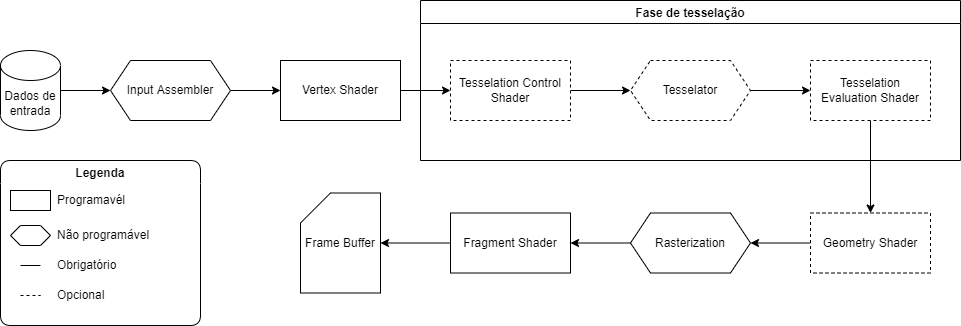
\includegraphics[width=1\textwidth]{imagens/PipelineRenderizacaoOpenGL.png}
\caption{Pipeline de Renderização Atual em OpenGL (Simplificado)}
\label{fig:LABEL_FIG_PIPELINE_ATUAL}
\end{figure}

\section{Compute Shaders}\label{sec:LABEL_CHP_1_SEC_C}

O \textit{compute shader} é um tipo especifico de shader que permite o processamento de grandes quantidades de dados arbitrários distribuídos entre diferentes grupos de trabalhos (\textit{workgroups}). Um workgroup é um conjunto de threads\footnote{Fluxo de execução independente de um programa} que compartilham uma memória de rápido acesso, conforme ilustrado na Figura \ref{fig:LABEL_FIG_WORKGROUPS}. Compute shaders melhor exploram as capacidades do hardware moderno ao flexibilizar a forma em que os dados são processados. O modelo de programação via workgroups permitem que informações transitem entre as unidades de processamento das GPUs sem que haja a necessidade da invocação de outros shaders, possibilitando a execução de algoritmos mais complexos. 

O paradigma computacional dos compute shaders se assemelha ao bibliotecas como OpenCL e CUDA. Entretanto, apesar de compute shaders não conter todas as funcionalidades, seu uso é vantajoso em aplicações em OpenGL pelos seguintes motivos:

\begin{itemize}
  \item Compute shaders são escritos em GLSL, similar à outros shaders escritos para OpenGL;
  \item A validação, compilação e montagem de computer shaders são realizadas da mesma forma que outros shaders em OpenGL;
  \item O uso de compute shaders não requer instalação e configuração de bibliotecas adicionais além do OpenGL 4.3+;
  \item Não há a necessidade de criação e liberação de novos contextos. Compute shaders utilizam o mesmo contexto que o pipeline de renderização do OpenGL.
\end{itemize}

\subsection{Leitura e Escrita de Dados}\label{sec:LAVEL_CHP_1_SEC_D}

Compute shaders permitem a leitura e escrita de informações através dos \textit{Shader Storage Buffer Object} (SSBO). Os SSBOs são estruturas que armazenam dados de forma similar aos \textit{uniforms} \ref{sec:LABEL_CHP_1_SEC_C}, porém diferentemente destes, eles podem possuir um tamanho muito maior além de poderem ser operados de maneira atômica (operações atômicas garantem a coerência das informações ao impedir que múltiplas threads atuem sobre o mesmo dado simultaneamente).

\begin{figure}
  \centering
  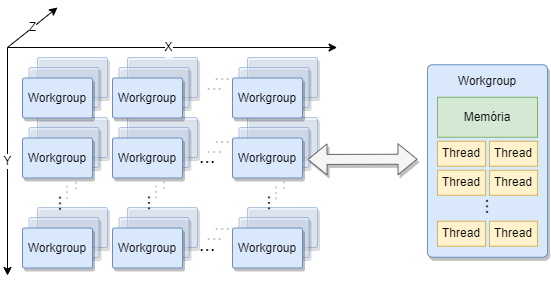
\includegraphics[width=0.75\textwidth]{imagens/WorkgroupsVisualisation2.drawio.png}
  \caption{Distribuição de workgroups e threads em Compute Shaders}
  \label{fig:LABEL_FIG_WORKGROUPS}
\end{figure}

\subsection{O problema da renderização indireta}\label{sec:LABEL_RENDERIZACAO_INDIRETA}

Ao finalizar a execução de um compute shader, as informações processadas podem ser resgatadas da memória de vídeo para a memória principal para serem tratadas pela CPU através dos SSBO. Caso haja a necessidade de utilizar essas informações durante o pipeline de renderização, esses dados necessitam ser repassados novamente à memória de vídeo utilizando \textit{uniforms} de entrada para a execução de um outro programa que contenha ao menos vertex e fragment shaders. Essa renderização indireta pode ser computacionalmente custosa por conta do overhead de transmissão dos dados entre as memórias de vídeo e principal.

\section{Mesh Shaders}\label{sec:LABEL_CHP_1_SEC_D}

Em poucas palavras, mesh shaders são compute shaders capazes de enviar geometrias primitivas diretamente para o rasterizador. Sendo possível realizar todas as funcionalidades que são implementadas do pipeline VTGS, como \textit{occlusion culling}, tesselação e \textit{instancing}, o pipeline que utiliza Mesh shaders é capaz de substituir por completo o pipeline de renderização atual, com a vantagem de ser mais simples e maleável.

Seu principal objetivo é simplificar a esteira de renderização ao remover a etapa de input assembler e integrar as funcionalidades de tesselation evaluation e geometry shaders às etapas iniciais do fluxo. Além disso, mesh shaders visam resolver o problema do gargalo da linearidade dos vertex e index buffers ao permitir que múltiplas subseções de uma malha sejam processadas em paralelo utilizando o conceito de \textit{meshlets}, permitindo assim que geometrias complexas sejam renderizadas de forma mais eficiente. ilustrado na Figura \ref{fig:LABEL_FIG_MESHLETS}.

\begin{figure}
  \centering
  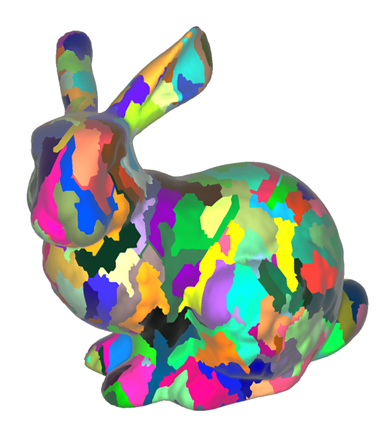
\includegraphics[width=0.25\textwidth]{imagens/MeshletsBunnyNVidia.png}
  \caption{Representação visual de uma geometria subdividida em \textit{meshlets}}
  \label{fig:LABEL_FIG_MESHLETS}
\end{figure}

Mesh shaders permitem que os desenvolvedores gerenciem melhor o uso dos recursos utilizados pelas GPUs. Diferentemente da esteira vigente, esta nova abordagem possibilita que um dado lido pela memória principal permaneça na memória de video até quando for necessário.

Dado seu modelo de computação similar aos compute shaders, mesh shaders facilitam a geração de malha procedural diretamente pela GPU. Processo este que era inflexível, limitado e não performático ao se utilizar TCS, TES e geometry shaders no pipeline VTGS.

Como restrição, Mesh shaders necessitam da alocação prévia de recursos em tempo de compilação. Durante a escrita código do shader, deve-se definir a quantidade de threads, o tipo de primitivo de saída e, por fim, o número máximo de primitivos e vértices gerados por workgroup. Além disso, a primeira geração de hardwares que suportam mesh shaders contém restritas limitações no número máximo de primitivos gerados por workgroup. Por conta disso, para evitar a alocação desnecessária de recursos, é desejável que se tenha um balanceamento entre estes parâmetros.

\subsection{Task Shaders}\label{sec:LAVEL_CHP_1_SEC_TASK_SHADERS}

O pipeline baseado em mesh shaders inclui uma extensão programável chamada de \textit{task shaders} (ou \textit{amplification shader}, em DirectX). Assim como ilustrado na Figura \ref{fig:LABEL_FIG_FLUXO_TASK_MESH_SHADERS}, task shaders são etapas que opcionais antecedem a execução de mesh shaders e tem como principal objetivo a gestão dinâmica de sua carga de trabalho. Task shaders, assim como mesh shaders, também possuem dados de entrada e saída definidas pelo usuário e trabalham com o conceito de workgroups como vistos em compute shaders.

Cada workgroup de um task shader pode ou não emitir uma instancia de mesh shader. Um exemplo de caso de uso é a implementação do \textit{occlusion culling} durante as etapas iniciais do pipeline. O occlusion culling é o processo que se refere à omissão de malha que não será exibida na imagem final, evitando eventuais desperdícios de processamento e no uso de recursos da GPU.

\begin{figure}
  \centering
  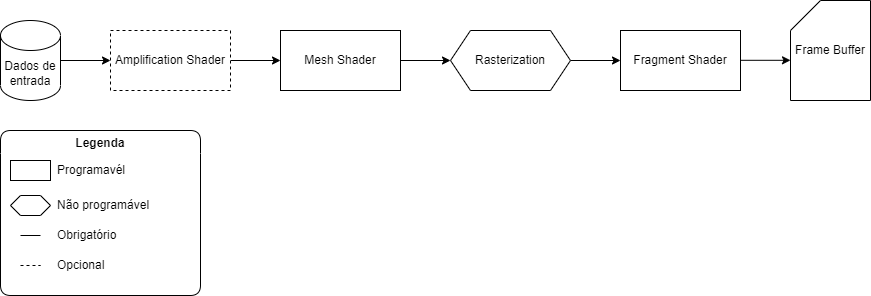
\includegraphics[width=1\textwidth]{imagens/PipelineRenderizacaoOpenGL-Mesh_Shader.png}
  \caption{Pipeline Utilizando Mesh Shaders}
  \label{fig:LABEL_FIG_FLUXO_TASK_MESH_SHADERS}
\end{figure}

%%\codec{Definições iniciais mesh shader}{alg:LABEL_CODE_1}{codigos/codigo-c.txt}


%%\textcolor{red}{TODO: Melhorar sessão de limitações}


%%\textcolor{red}{TODO: Organizar e melhorar figuras}